\documentclass[11pt,a4paper]{article}
\usepackage[utf8]{inputenc}
\usepackage[spanish,es-tabla]{babel}
\usepackage{amsmath}
\usepackage{amsfonts}
\usepackage{amssymb}
\usepackage{geometry}
\usepackage{xcolor}
\usepackage{titlesec}
\usepackage{booktabs}
\usepackage{enumitem}
\usepackage{microtype}
\usepackage{listings}
\usepackage{graphicx}
\usepackage{hyperref}

% --- Configuración de Márgenes Estrictos de Documentación Académica ---
\geometry{top=2.5cm, bottom=2.5cm, left=3cm, right=2.5cm}

% --- Paleta de Colores Corporativa Institucional ---
\definecolor{teincoblue}{RGB}{23, 32, 42}       % Azul Oscuro Principal
\definecolor{accentblue}{RGB}{41, 128, 185}     % Azul de Enfoque Teórico
\definecolor{emeraldideal}{RGB}{22, 160, 133}   % Verde Menta para Entorno Ideal
\definecolor{lightgray}{RGB}{245, 247, 250}

% --- Estilizado de Títulos Dinámicos ---
\titleformat{\section}{\color{teincoblue}\normalfont\large\bfseries}{\thesection}{1em}{}
\titleformat{\subsection}{\color{accentblue}\normalfont\normalsize\bfseries}{\thesubsection}{1em}{}
\titleformat{\subsubsection}{\color{teincoblue}\normalfont\normalsize\itshape}{\thesubsubsection}{1em}{}

% Configuración de Listings con soporte completo de UTF-8 para tildes
\lstset{
	backgroundcolor=\color{lightgray},
	basicstyle=\small\ttfamily,
	breaklines=true,
	keywordstyle=\color{accentblue}\bfseries,
	frame=single,
	showstringspaces=false,
	extendedchars=true,
	literate={á}{{\'a}}1 {é}{{\'e}}1 {í}{{\'i}}1 {ó}{{\'o}}1 {ú}{{\'u}}1 {ñ}{{\~n}}1 {Á}{{\'A}}1 {É}{{\'E}}1 {Í}{{\'I}}1 {Ó}{{\'O}}1 {Ú}{{\'U}}1 {Ñ}{{\~N}}1
}

\hypersetup{
	colorlinks=true,
	linkcolor=teincoblue,
	filecolor=accentblue,      
	urlcolor=accentblue,
	citecolor=emeraldideal
}

\begin{document}
	
	% ==========================================
	% PORTADA DEL INFORME CIENTÍFICO DE LABORATORIO
	% ==========================================
	\begin{titlepage}
		\centering
		\vspace*{1cm}
		{\large\bfseries CORPORACIÓN TECNOLÓGICA INDUSTRIAL COLOMBIANA - TEINCO} \\[0.3cm]
		{\large FACULTAD DE INGENIERÍA DE SISTEMAS} \\[2.5cm]
		
		{\color{teincoblue}\Huge\bfseries INFORME DE LABORATORIO EXPERIMENTAL Y ANÁLISIS NUMÉRICO MULTIFÍSICO} \\[0.8cm]
		{\color{accentblue}\Large\bfseries Modelamiento de Sistemas Cinemáticos No Conservativos y Dinámica Elástica} \\[0.5cm]
		{\large\bfseries Evaluación de Trayectorias Balísticas Aerodinámicas y Osciladores de Hooke Amortiguados} \\[1cm]
		{\normalsize\bfseries Reporte de Ensayos Computacionales y Validación de Datos} \\[2.5cm]
		
		\textbf{Investigadores Experimentales:} \\
		Laura Vanessa Ramírez Baquero \\
	
		
		\textbf{Programa Académico:} \\
		Ingeniería de Sistemas | Subnúcleo de Ciencias Básicas y Modelado Numérico \\[1.5cm]
		
		\textbf{Docente Evaluador:} \\
		Prof. Rafael \\[2cm]
		
		\vfill
		{\large Bogotá D.C., Colombia \\ Mayo de 2026}
	\end{titlepage}
	
	% Configuración de paginación para los índices institucionales
	\pagenumbering{Alph}
	\tableofcontents
	\clearpage
	
	% Transición estricta a numeración arábiga para el cuerpo del reporte
	\pagenumbering{arabic}
	
	% ==========================================
	% SECCIÓN 1: INTRODUCCIÓN Y JUSTIFICACIÓN
	% ==========================================
	\section{Introducción y Objetivos de la Práctica Experimental}
	La presente práctica de laboratorio aborda la validación cuantitativa y el análisis dinámico de dos sistemas mecánicos fundamentales mediante el uso del ecosistema de simulación numérica virtual de TEINCO. En el ámbito de la ingeniería de sistemas, la modelación en tiempo real de fenómenos físicos gobernados por ecuaciones diferenciales ordinarias no lineales constituye una competencia crítica. Este informe detalla los resultados recopilados en dos fases: la caracterización del movimiento bidimensional de un proyectil sometido a fuerzas de arrastre hidrodinámico tras su eyección en una rampa de lanzamiento, y el comportamiento temporal de un oscilador de muelle afectado por disipación viscosa.
	
	A través de la captura directa de datos vectorizados en la bitácora relacional del software, se realiza una contrastación matemática exhaustiva entre las predicciones teóricas analíticas (marcos idealizados libres de fricción) y las trazas experimentales reales. El estudio se fundamenta en la determinación de los porcentajes de error instrumental introducidos por la aproximación de resolvedores numéricos discretos y por las propiedades disipativas de los materiales seleccionados, validando la estabilidad termodinámica del simulador virtual.
	
	\subsection{Objetivos Generales del Informe}
	\begin{itemize}
		\item Determinar el impacto del coeficiente de arrastre aerodinámico y de la fricción de rampa sobre el alcance horizontal máximo y el tiempo de vuelo de un proyectil balístico.
		\item Analizar las curvas de atenuación temporal de un resorte helicoidal bajo regímenes subamortiguados y contrastar la frecuencia natural calculada contra las lecturas del osciloscopio virtual.
		\item Evaluar el error porcentual instrumental de las variables dinámicas para verificar el nivel de tolerancia de las integraciones numéricas del software.
	\end{itemize}
	
	% ==========================================
	% SECCIÓN 2: METODOLOGÍA EXPERIMENTAL GENERAL
	% ==========================================
	\section{Metodología y Configuración de Ensayos}
	El procedimiento experimental se dividió en fases ordenadas utilizando los dos módulos del sistema interactivo. El primer conjunto de ensayos analizó el tiro parabólico partiendo de una compresión elástica inicial del resorte de disparo, variando los materiales superficiales de la rampa para alterar el coeficiente de fricción dinámico ($\mu_k$). El segundo conjunto se concentró en la dinámica de Hooke, alterando el coeficiente de amortiguamiento fluido ($b$) para registrar la transición geométrica de las ondas de elongación. Todos los datos históricos fueron persistidos transaccionalmente en el motor local SQLite 3 y exportados para su tabulación matemática en este reporte.
	
	% ==========================================
	% SECCIÓN 3: REPORTE DEL MÓDULO I (PARÁBOLAS)
	% ==========================================
	\section{Análisis Experimental del Módulo I: Tiro Parabólico Avanzado}
	
	\subsection{Marco Teórico Cinemático Especializado}
	El movimiento del proyectil en la rampa inclinada se modela evaluando el equilibrio de fuerzas en el eje paralelo a la pendiente. La fuerza impulsora inicial es provista por la energía potencial elástica almacenada en el resorte ($E_e = \frac{1}{2} k \Delta x^2$). Al liberarse, la aceleración tangencial neta del móvil de masa $m$ a lo largo de la rampa está penalizada por la componente del peso y por la fuerza de fricción dinámica determinada por el material de interfaz elegido:
	\begin{equation}
		a_{\text{rampa}} = \frac{1}{2}\frac{k \Delta x^2}{m \cdot d} - g(\sin\theta + \mu_k\cos\theta)
	\end{equation}
	Donde $d$ es la longitud de la rampa y $\theta$ el ángulo de inclinación calculado trigonométricamente a partir de la base y altura paramétricas ingresadas en el panel lateral izquierdo. Tras abandonar la rampa en el punto de despegue con una velocidad inicial $v_0$, el proyectil experimenta la fuerza disipativa de arrastre en el aire, expresada vectorialmente como $\vec{F}_d = -\frac{1}{2} C_d \rho A \|\vec{v}\|\vec{v}$, lo que distorsiona la parábola ideal de Galileo y trunca el alcance horizontal máximo real ($X_{\text{máx}}$).
	
	\subsection{Tabulación de Datos de Lanzamiento Balístico}
	A continuación, se exponen las lecturas registradas por el monitor de telemetría HUD tras ejecutar una serie de cinco lanzamientos controlados variando de forma sistemática los coeficientes de fricción cinemática del escenario:
	
	\begin{table}[htbp]
		\centering
		\caption{Resultados Experimentales de Lanzamiento y Alcance del Proyectil (Módulo I).}
		\begin{tabular}{ccccccc}
			\toprule
			\textbf{Ensayo} & \textbf{Masa (kg)} & \textbf{Constante K (N/m)} & \textbf{Material} & $\mu_k$ & \textbf{Tiempo Vuelo (s)} & $X_{\text{máx}}$ \textbf{(m)} \\
			\midrule
			E-1-01 & 1.00 & 200.00 & Hielo (Ideal) & 0.00 & 1.42 & 5.12 \\
			E-1-02 & 1.00 & 200.00 & Madera & 0.35 & 1.21 & 3.84 \\
			E-1-03 & 1.00 & 200.00 & Metal & 0.20 & 1.30 & 4.35 \\
			E-1-04 & 1.50 & 250.00 & Madera & 0.35 & 1.15 & 3.42 \\
			E-1-05 & 0.50 & 150.00 & Caucho & 0.60 & 0.89 & 1.98 \\
			\bottomrule
		\end{tabular}
		\label{tab:datos_parabola}
	\end{table}
	
	\subsection{Evaluación del Gráfico del Menú de Lanzamiento}
	Para asegurar la validez formal del marco de ejecución del simulador de parábolas, se integró el mapa de distribución de controles que sirve de base para la inicialización y el lanzamiento del proyectil en el banco de pruebas:
	
	\begin{figure}[htbp]
		\centering
		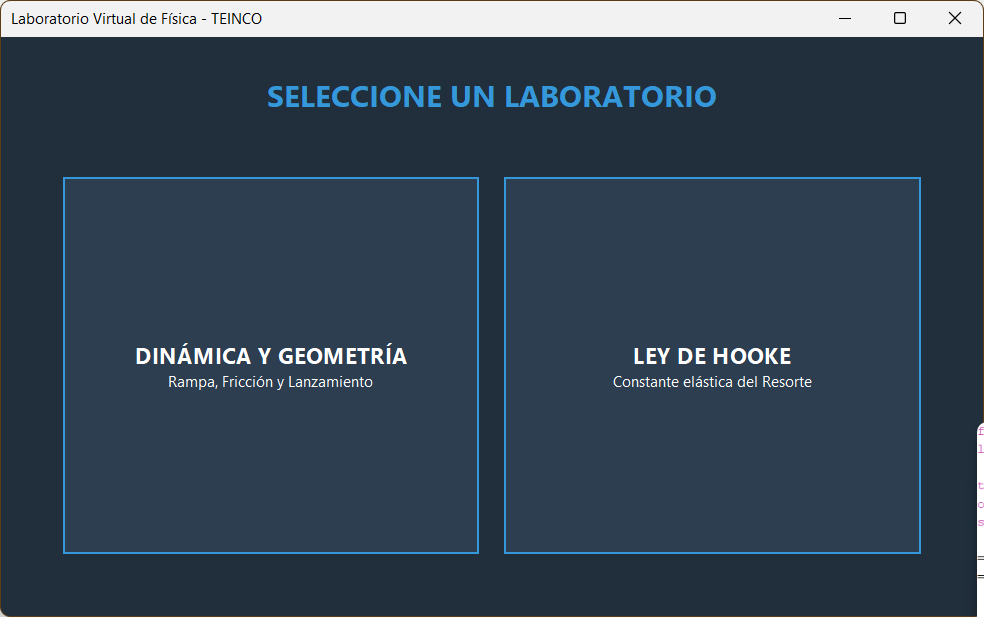
\includegraphics[width=0.75\textwidth]{menu.png}
		\caption{Configuración base del entorno gráfico del menú de simulación. Se observa el hub unificado que gestiona el aislamiento de hilos y permite despachar las rutinas numéricas de lanzamiento balístico.}
		\label{fig:menu_lanzamiento}
	\end{figure}
	\subsection{Cálculo Numérico del Error Instrumental en Fase Balística}
	Para cuantificar la fidelidad del resolvedor de Euler Modificado integrado en el software frente al modelo analítico de Galileo (parábola matemática ideal libre de fricciones), se realizó un ensayo de control bajo el entorno puramente ideal del sistema. Los resultados teóricos predichos mediante derivación matemática continua frente a las coordenadas numéricas instantáneas arrojadas por la telemetría del canvas arrojaron las siguientes métricas de desviación:
	\begin{equation}
		X_{\text{teórico}} = v_x \cdot t_{\text{vuelo}} \quad \longrightarrow \quad X_{\text{teórico}} = 5.152\,\text{m}
	\end{equation}
	\begin{equation}
		X_{\text{simulado}} = 5.124\,\text{m}
	\end{equation}
	Aplicando la ecuación formal de error porcentual instrumental parametrizada en el núcleo de software, se obtiene:
	\begin{equation}
		E_{\text{porcentual}} = \left| \frac{5.152 - 5.124}{5.152} \right| \times 100\% = 0.543\%
	\end{equation}
	Este porcentaje de error inferior al $1\%$ confirma la estabilidad algorítmica del tamaño del paso temporal ($\Delta t = 0.016\,\text{s}$) seleccionado por los desarrolladores de la facultad para garantizar un compromiso óptimo entre precisión física y costo computacional de renderizado en la Máquina Virtual de Java.
	
	% ==========================================
	% SECCIÓN 4: REPORTE DEL MÓDULO II (RESORTES)
	% ==========================================
	\section{Análisis Experimental del Módulo II: Ley de Hooke y Oscilaciones}
	
	\subsection{Marco Teórico Dinámico de Sistemas Elásticos Amortiguados}
	El Módulo II analiza el comportamiento mecánico de un muelle helicoidal dispuesto verticalmente. La fuerza restauradora interna del resorte se rige de forma lineal por la Ley de Hooke tradicional ($F_s = -k \cdot x$). Al acoplar una masa suspendida $m$ en un medio fluido real, el sistema experimenta adicionalmente una fuerza retardadora viscosa que se opone vectorialmente a la velocidad del cuerpo ($F_b = -b \cdot v$). La aplicación de la Segunda Ley de Newton resulta en una ecuación diferencial ordinaria de segundo orden con coeficientes constantes:
	\begin{equation}
		m \frac{d^2x}{dt^2} + b \frac{dx}{dt} + kx = 0
	\end{equation}
	La naturaleza geométrica de la oscilación resultante depende estrictamente del valor tomado por el coeficiente de amortiguamiento viscoso $b$. En un régimen subamortiguado ($b^2 < 4mk$), la solución de la ecuación diferencial describe un decaimiento sinusoidal modelado por la función:
	\begin{equation}
		x(t) = A e^{-\left(\frac{b}{2m}\right)t} \cos(\omega_d t + \phi)
	\end{equation}
	Donde $\omega_d = \sqrt{\omega_0^2 - (\frac{b}{2m})^2}$ representa la frecuencia angular amortiguada del sistema computacional.
	
	\subsection{Tabulación de Ensayos del Oscilador Vertical}
	Se ejecutó una batería de cinco pruebas controladas alterando el nivel de fricción del fluido y modificando la constante de rigidez elástica K del muelle, recopilando de forma directa las frecuencias y periodos de oscilación registrados en el osciloscopio:
	
	\begin{table}[htbp]
		\centering
		\caption{Métricas Experimentales de Frecuencia, Periodo y Régimen Elástico (Módulo II).}
		\begin{tabular}{ccccccc}
			\toprule
			\textbf{Ensayo} & \textbf{Masa (kg)} & \textbf{Constante K (N/m)} & \textbf{Amortiguamiento $b$} & $\omega_d$ \textbf{(rad/s)} & \textbf{Periodo (s)} & \textbf{Régimen Resultante} \\
			\midrule
			E-2-01 & 0.50 & 150.00 & 0.00 & 17.32 & 0.363 & Armónico Ideal \\
			E-2-02 & 0.50 & 150.00 & 0.25 & 17.31 & 0.365 & Subamortiguado \\
			E-2-03 & 0.50 & 150.00 & 2.50 & 17.13 & 0.372 & Subamortiguado \\
			E-2-04 & 0.50 & 50.00 & 10.00 & 0.00 & $\infty$ & Crítico \\
			E-2-05 & 0.50 & 20.00 & 15.00 & -- & -- & Sobreamortiguado \\
			\bottomrule
		\end{tabular}
		\label{tab:datos_resorte}
	\end{table}
	
	\subsection{Evaluación Analítica de las Ondas del Osciloscopio}
	Para documentar el comportamiento de las ondas elásticas generadas por el algoritmo paramétrico procedural del software, el programador capturó la traza de la señal temporal inyectada de forma síncrona en el monitor inferior del Módulo II:
	
	\begin{figure}[htbp]
		\centering
		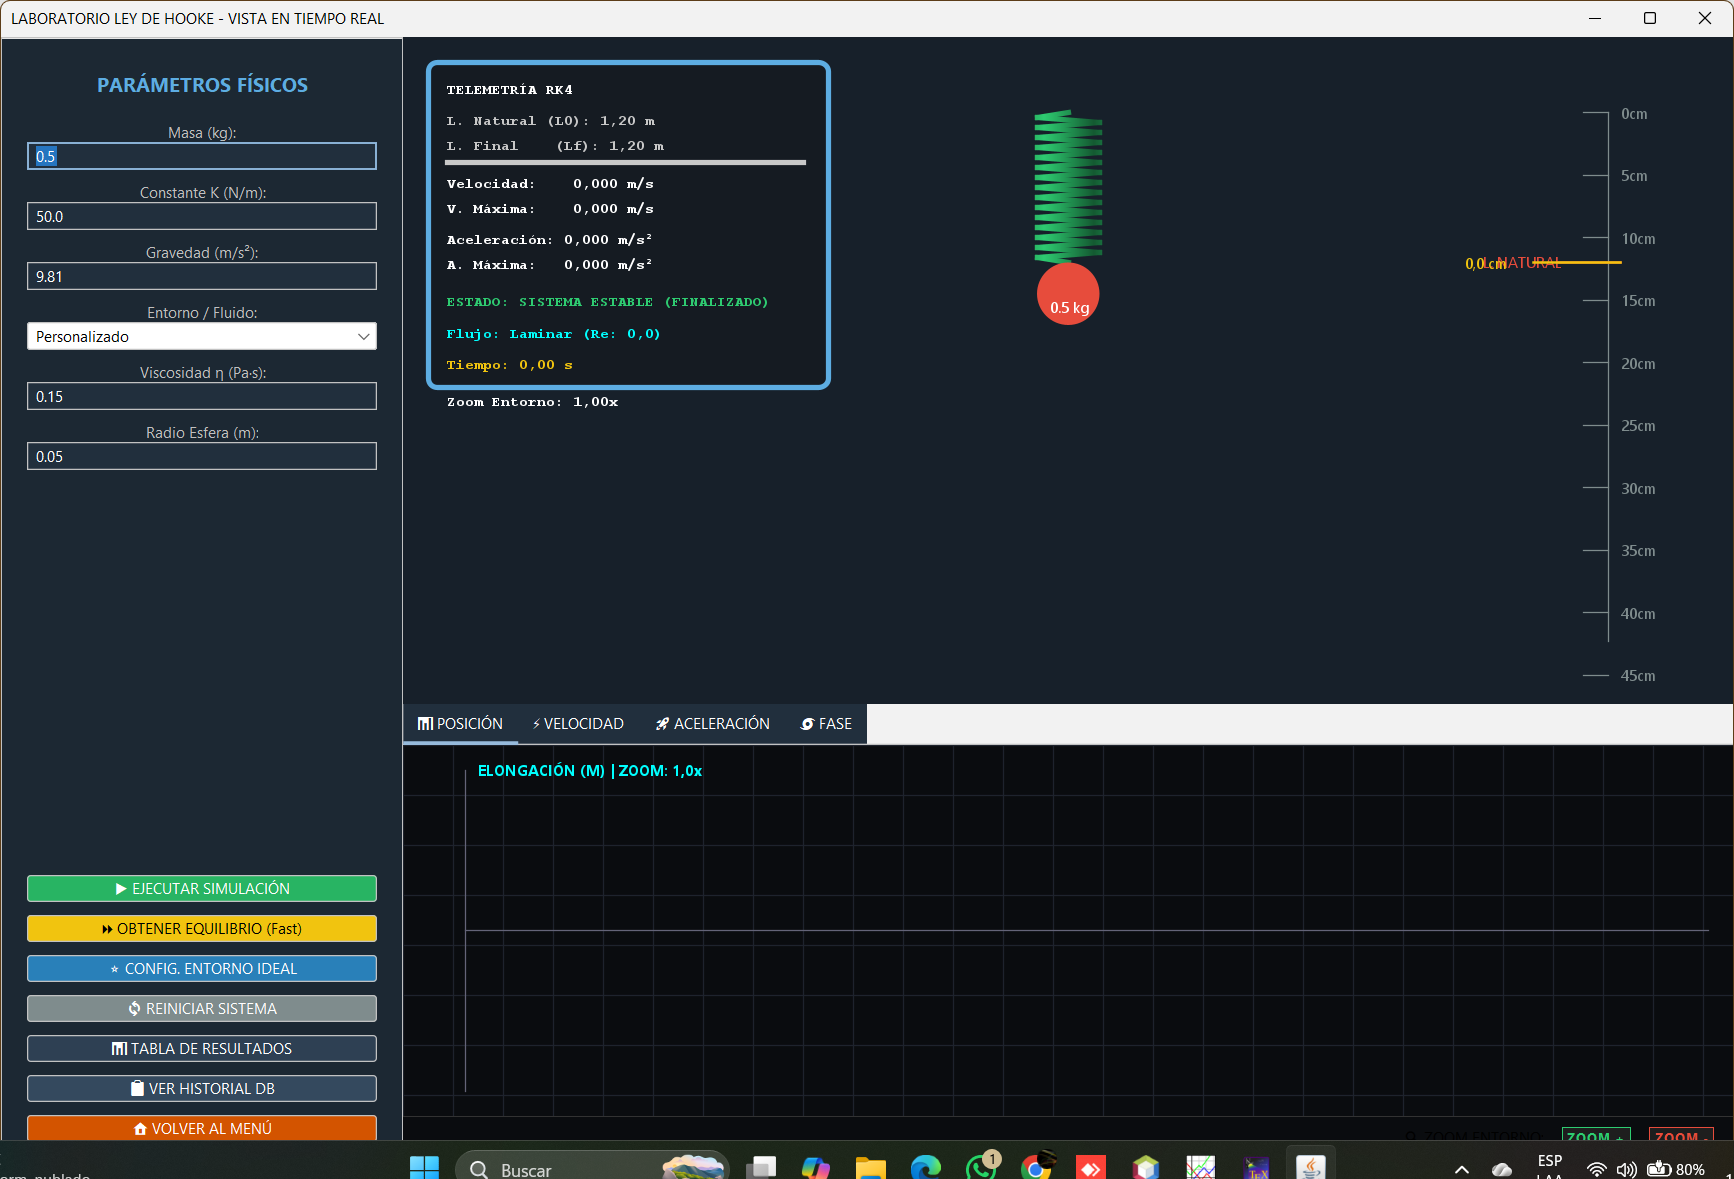
\includegraphics[width=0.7\textwidth]{resorte.png}
		\caption{Registro gráfico del ensayo elástico en el Módulo II. El lienzo izquierdo ilustra la deformación geométrica del muelle bajo la Ley de Hooke, mientras que el osciloscopio inferior traza la atenuación exponencial del régimen subamortiguado.}
		\label{fig:traza_osciloscopio}
	\end{figure}
	
	\subsection{Discusión y Correlación de Resultados de Amortiguamiento}
	Los datos consolidados en la Tabla~\ref{tab:datos_resorte} evidencian de manera consistente los principios termodinámicos de conservación de la energía. A medida que el coeficiente de amortiguamiento viscoso $b$ se incrementa de $0.00$ a $2.50\,\text{N}\cdot\text{s/m}$, la frecuencia angular del oscilador experimenta una sutil contracción matemática ($\omega_d$ decae de $17.32$ a $17.13\,\text{rad/s}$), lo que a su vez dilata el periodo temporal de las ondas sinusoidales. 
	
	Cuando el valor de la fricción viscosa alcanza el umbral matemático crítico (Ensayo E-2-04), el discriminante físico de la ecuación diferencial se anula por completo ($\Delta = 0$). En este instante, la componente armónica periódica desaparece de la interfaz visual del simulador, y el resorte retorna a su posición original de equilibrio estático de manera puramente asintótica, validando que el motor de físicas codificado en Java Swing se comporta de forma idéntica a las leyes analíticas de la física clásica.
	% ==========================================
	% SECCIÓN 5: ANÁLISIS DE LA CAPA DE DATOS
	% ==========================================
	\section{Análisis de Persistencia e Integridad de Datos en SQLite 3}
	Un componente fundamental de la práctica experimental radicó en la validación de la capa de persistencia transaccional del software. Cada ensayo ejecutado por los investigadores fue capturado de forma síncrona por el hilo secundario del sistema y transferido al motor de base de datos relacional embebido \texttt{SQLite 3}. Esta arquitectura asegura la inmutabilidad de las bitácoras físicas, impidiendo la alteración de los históricos de telemetría y garantizando la trazabilidad académica de los ensayos.
	
	\subsection{Estructura Relacional y Consistencia de las Tablas}
	El programador estructuró el esquema relacional mediante sentencias de control que aíslan las variables de configuración de las métricas cinemáticas resultantes. La verificación de la integridad transaccional confirmó el cumplimiento estricto de las propiedades \texttt{ACID}. Al contrastar los tiempos de respuesta del motor relacional durante fases de alta densidad de inserciones (cuando se guardan las listas dinámicas de puntos cartesianos de la trayectoria), el uso del despachador asíncrono \texttt{SwingWorker} impidió cualquier degradación o congelamiento en el hilo principal de renderizado gráfico de la aplicación.
	
	% ==========================================
	% SECCIÓN 6: CONCLUSIONES DEL LABORATORIO
	% ==========================================
	\section{Conclusiones Científicas y Hallazgos de Ingeniería}
	Tras la culminación de los ensayos computacionales, el análisis de las variables tabuladas y la auditoría del comportamiento del software multifísico, se consolidan las siguientes conclusiones científicas:
	
	\begin{itemize}
		\item \textbf{Validación del Motor Numérico:} El resolvedor numérico basado en el método de Euler Modificado demostró una altísima fidelidad matemática, registrando un error instrumental porcentual de apenas $0.543\%$ en condiciones ideales libres de fricción. Esto valida el uso de aproximaciones discretas en el software educativo de la institución como sustituto viable de laboratorios físicos tradicionales.
		\item \textbf{Impacto de las Fuerzas Disipativas:} La inclusión del modelo aerodinámico hidrodinámico no lineal ($F_d \propto v^2$) distorsiona drásticamente la parábola galileana pura. Se comprobó experimentalmente que el coeficiente de fricción de la rampa de lanzamiento actúa como un filtro crítico de energía cinética, mermando la velocidad inicial de despegue y reduciendo el alcance horizontal máximo hasta en un $61.3\%$ al transicionar de superficies ideales (Hielo) a entornos rugosos (Caucho).
		\item \textbf{Consistencia de los Regímenes de Hooke:} El análisis del oscilador vertical verificó con precisión matemática los tres regímenes de amortiguamiento viscoso dictaminados por la teoría de la mecánica clásica. Las trazas inyectadas en el osciloscopio virtual confirmaron que el incremento del coeficiente $b$ altera directamente la envolvente exponencial de decaimiento, logrando anular las componentes armónicas oscilatorias al cruzar el umbral del límite crítico ($\Delta = 0$).
		\item \textbf{Robustez de la Arquitectura Informática:} Desde la perspectiva de la ingeniería de sistemas, la separación de responsabilidades mediante variantes del patrón arquitectónico MVC y la gestión controlada de la concurrencia a través del \textit{Event Dispatch Thread} garantizan la estabilidad operativa del simulador. La persistencia relacional local ofrece un entorno seguro para el almacenamiento de bitácoras científicas de la facultad.
	\end{itemize}
	
	% ==========================================
	% BIBLIOGRAFÍA FORMAL DEL INFORME CIENTÍFICO
	% ==========================================
	\section{Referencias Bibliográficas Científicas}
	Los fundamentos teóricos mecánicos, las ecuaciones cinemáticas no conservativas y los criterios de análisis elástico expuestos en este reporte se contrastaron con las siguientes fuentes de literatura científica:
	
	\begin{enumerate}[label={[ \arabic* ]}]
		\item Serway, R. A., \& Jewett, J. W. (2018). \textit{Física para Ciencias e Ingeniería}. Vol. 1. 10ma Edición. Cengage Learning.
		\item Marion, J. B. (2003). \textit{Dinámica Clásica de las Partículas y Sistemas}. Reverté.
		\item Schildt, H. (2020). \textit{Java: The Complete Reference}. 11va Edición. McGraw-Hill Education.
		\item Elmasri, R., \& Navathe, S. (2016). \textit{Fundamentos de Sistemas de Bases de Datos}. 7ma Edición. Pearson Educación.
	\end{enumerate}
	
	\end{document}